\chapter{制作PBR纹理的实用指南}

基于物理的渲染(Physically Based Rendering, PBR)与其被看做一个硬性标准,还不如说是一个方法论。它有具体的原则和参考,但是并不是一个真正的标准规范,而且会有不同的实现方式。这些区别通常体现在使用了不同的贴图类型(即所谓的工作流)、BRDF函数和粗糙度/光泽度的数据表达方式等。甚至有些实现会使用不同的映射名字,但用起来还是一样的。

在本文,我们将讨论两种最常见的工作流,即图\ref{fig:chap2_1}中的金属度/粗糙度工作流和高光/光泽度工作流。Substance工具套装中可用来处理PBR贴图的Sbustance Designer,Substance Painter和Bitmap2Material 3都支持这两种。针对这两种工作流的Substance PBR shaders使用了GGX BRDF,而且没有对输入的参数进一步处理或变换。但是如果需要自定义参数的话,利用Substance材质可以很方便的实现。更进一步来说,Substance工具套装中支持自定义shader,意味着你能将其修改至适应任意管线。

\begin{figure}[ht]
    \centering
	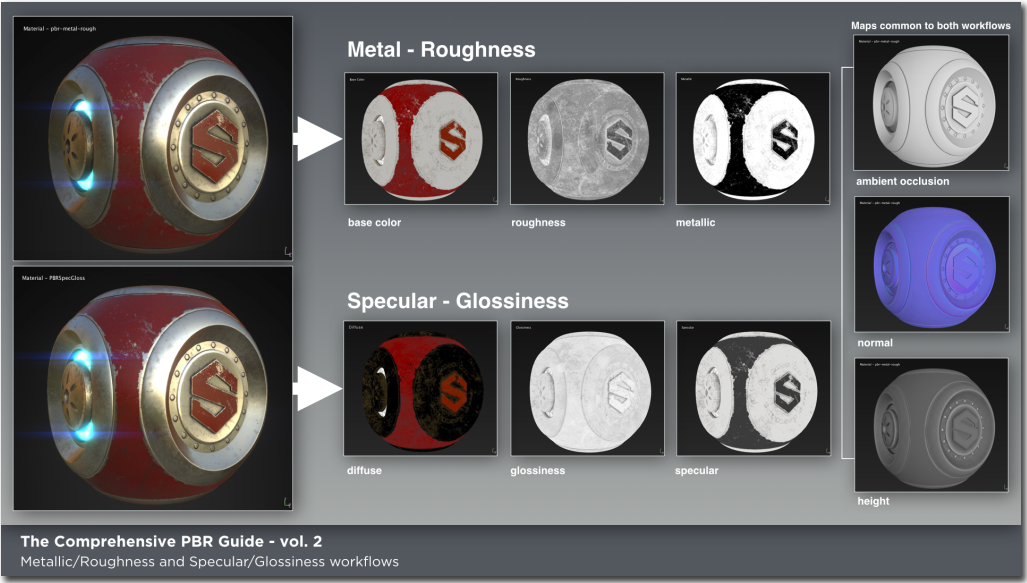
\includegraphics[width=\textwidth]{images/chap2_1.png}
	\caption{金属度/粗糙度工作流和高光/光泽度工作流}
    \label{fig:chap2_1}
\end{figure}

\section{什么是PBR?}

基于物理的渲染(PBR)是一个渲染方法,它可以更加精确的表现光照如何和表面交互。这个也可以被称为基于物理的光照(Physically Based Shading, PBS)。根据讨论的管线领域,PBS一般特指光照部分,而PBR特指渲染和光照。需要注意的是这两个东西其实都是从一个物理更加精确的角度来描述资源。

\subsection{PBR有什么好处?}

我们能从艺术家的角度和生产效率出发,得到PBR的好处

\begin{enumerate}
\item 我们能够更加轻松的制作真实资源,因为我们不需要去猜测诸如高光等表面属性,而可以通过物理正确的公式和算法来得到对应的值。
\item 资源在各个光照环境下都看起来正确。
\item 不同艺术家也能通过这一工作流制作出画风一致的作品。
\end{enumerate}

\subsection{对艺术家来说这意味什么?}

\textbf{作为艺术家,我们对描述表面属性的贴图有不同的理解。对于新的贴图类型有不同的规则需要遵守。}

我们需要从传统的渲染工作流经验里抛弃漫反射和高光贴图的概念。这些贴图现在只是用来表示光照环境下材质的一个近似。计算机硬件和渲染技术的发展使得我们能够更加精确的模拟光的物理性质。

在PBR中,shader能够通过能量手和和BRDF函数模拟更加复杂的物理性质,因此艺术家需要根据物理性质来绘制贴图。这样我们就能够节约猜测材质属性的时间,将精力投入到艺术创作方面。虽然参考规则来正确绘制贴图非常重要,这并不意味着我们需要抛弃艺术创作部分。事实上从一个艺术家的角度,制作材质的时候更要考虑其背后的故事,并通过细节来表现出来。不要被物理限制住手脚是非常重要的。正是因为我们在一个更加物理正确的环境下工作,这并不是说不能使用个性化的艺术手法。例如迪斯尼的基于物理的反射模型是被设计成『principled』模型,这意味着它更加贴近于艺术家的角度而不是严格物理模型。所以说我们应该掌握主要原则和知道,但不是成为其奴隶。

\section{金属度/粗糙度工作流}

金属度/粗糙度工作流是通过一些通道的集合来定义的,这些通道作为PBR Shader里的纹理传入。具体来说有固有色、金属度和粗糙度三张,如图\ref{fig:chap2_2}所示,具体每张贴图会在后面的章节里详细讨论。PBR Shader也能够支持环境遮挡、法线贴图和视差贴图等,如图\ref{fig:chap2_3}所示。这些贴图在不同的工作流中都会共用,将在\ref{sec:common_maps}节讨论。

在金属度/粗糙度工作流工作流中,金属本身的反射率体现在固有色贴图,而绝缘体的反射和掠射角的反射通过BRDF来处理。金属度贴图有点类似一个区分固有色贴图中金属和绝缘体部分的遮罩层。介质F0并不是手工指定的,而是通过shader处理。当shader发现金属度贴图是黑色时,它将固有色贴图对应区域视作绝缘体,使用4\%作为反射率(如图\ref{fig:chap2_4}所示)。正如我们在前文讨论,4\%这个值能够覆盖绝大多数常见绝缘体。需要注意的是,诸如介质F0、金属反射度和固有色亮度范围是从实际测量数据获得的。当我们讨论不同类型贴图时,制作指导是基于测量数据。

在前文我们讨论了能量守恒,也就是表面反射出的光不会比照射进来的更强。在具体实现中,shader会负责控制能量守恒,(Substance也是这么处理的)。使用金属度/粗糙度工作流实际上是无法打破能量守恒的。漫反射和高光通过金属度贴图来控制比例,这意味着你无法分别控制漫反射和高光从而产生比接收到的光更强的反射/折射效果。

\textbf{金属的反射和绝缘体的折射都被保存在固有色贴图中。}

\begin{figure}[ht]
    \centering
	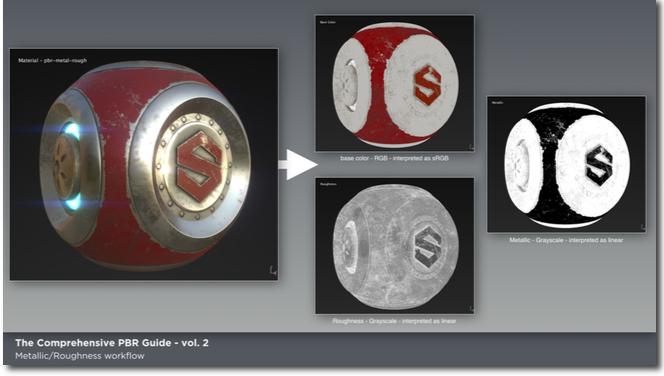
\includegraphics[width=\textwidth]{images/chap2_2.png}
	\caption{金属度/粗糙度工作流}
    \label{fig:chap2_2}
\end{figure}

\begin{figure}[ht]
    \centering
	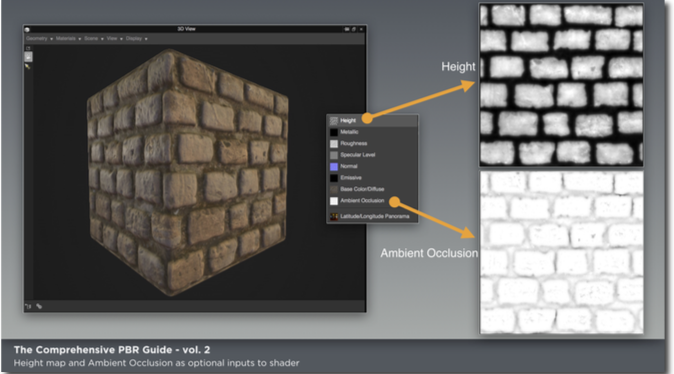
\includegraphics[width=\textwidth]{images/chap2_3.png}
	\caption{金属度/粗糙度工作流}
    \label{fig:chap2_3}
\end{figure}

\begin{figure}[ht]
    \centering
	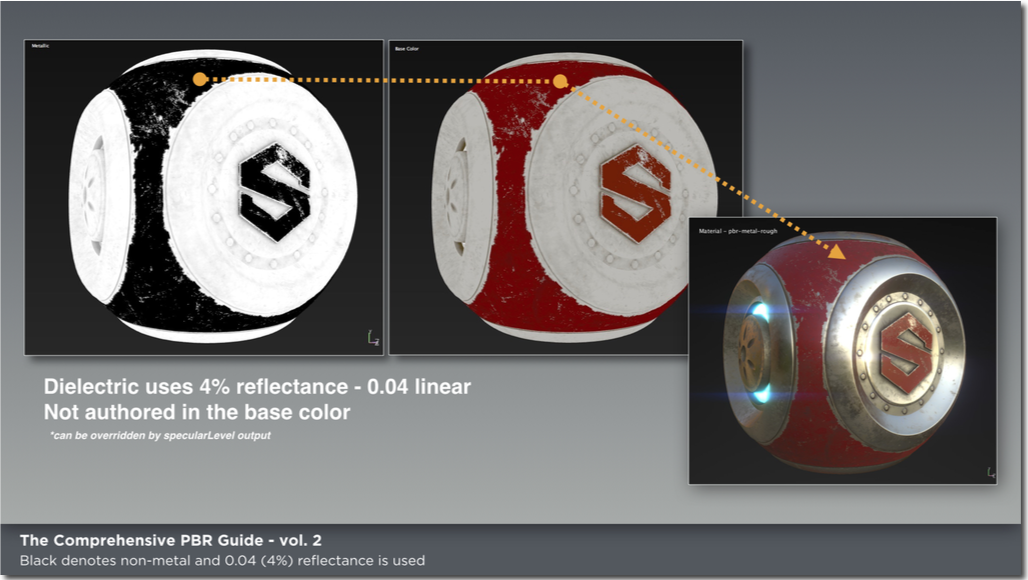
\includegraphics[width=\textwidth]{images/chap2_4.png}
	\caption{绝缘体使用4\%反射率,与固有色无关}
    \label{fig:chap2_4}
\end{figure}

\subsection{介质F0}

包括Substance和Unreal Engine 4在内的一些金属度/粗糙度工作流实现中提供了高光控制,这样艺术家就能够调整绝缘体的常量F0值。在Substance中,这个被标记为"specularLevel",通过纹理采样器提供。图\ref{fig:chap2_5}中展示了0.0-0.08范围。如果你需要手动调整绝缘体F0,直接修改Substance Designer中的"specularLevel"即可,如图\ref{fig:chap2_6}所示。我们将在高光/光滑度工作流中具体讨论F0。

\begin{figure}[ht]
    \centering
	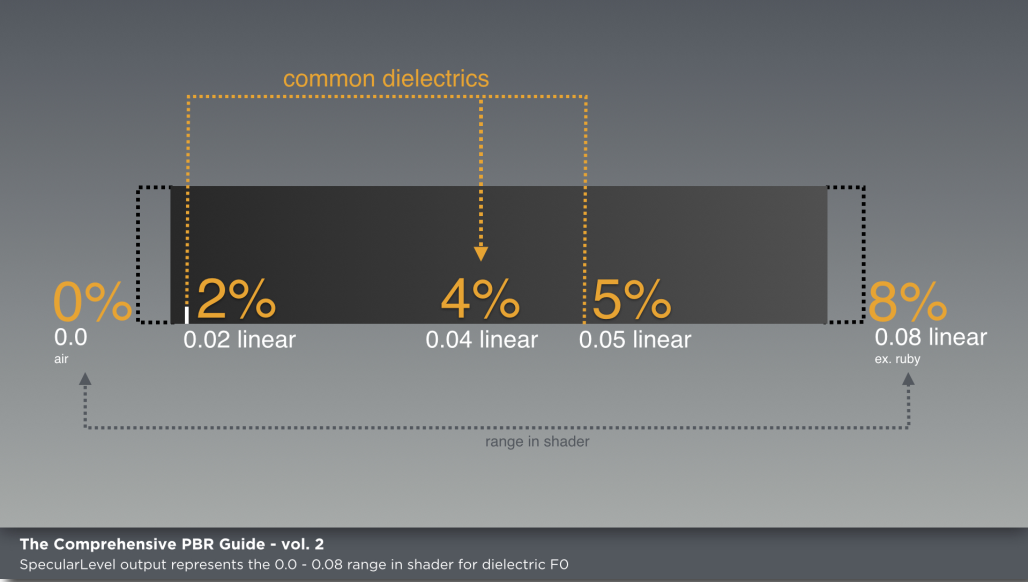
\includegraphics[width=\textwidth]{images/chap2_5.png}
	\caption{"specularLevel"代表shader中介质F0的0.0-0.08范围}
    \label{fig:chap2_5}
\end{figure}

\begin{figure}[ht]
    \centering
	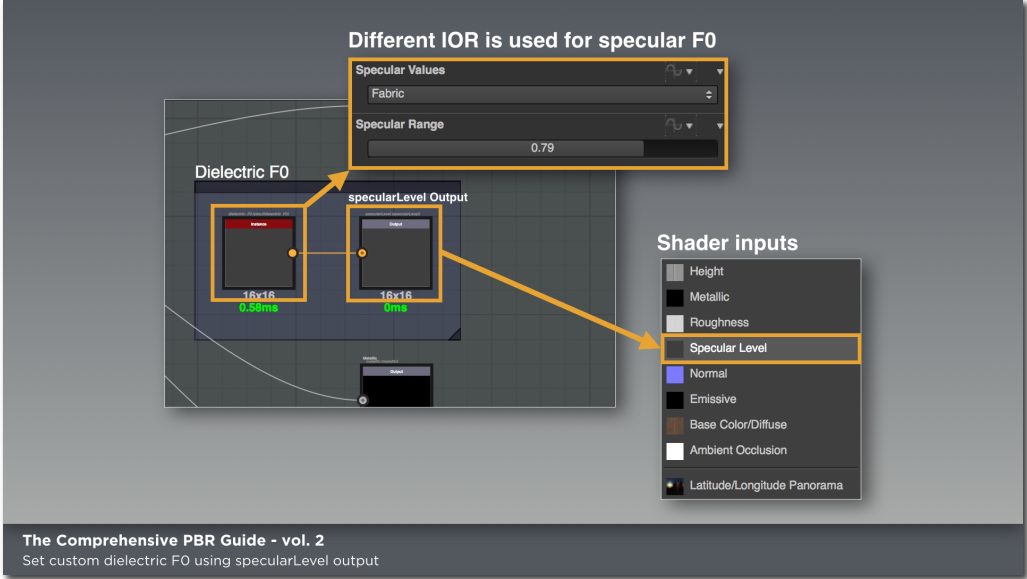
\includegraphics[width=\textwidth]{images/chap2_6.png}
	\caption{通过"specularLevel"设置自定义介质F0}
    \label{fig:chap2_6}
\end{figure}

\textbf{如果你需要手动设置绝缘体F0,你可以在Substance Designer里设置"specularLevel"。}

\subsection{固有色(RGB-sRGB)}

固有色贴图本质上是一个RGB贴图,其中包含了两类数据:绝缘体的反射颜色和金属的反射率,如图\ref{fig:chap2_7}所示。绝缘体的反射颜色表示反射的波长;如果金属度贴图中标记为金属,则对应的是反射率。

\begin{figure}[ht]
    \centering
	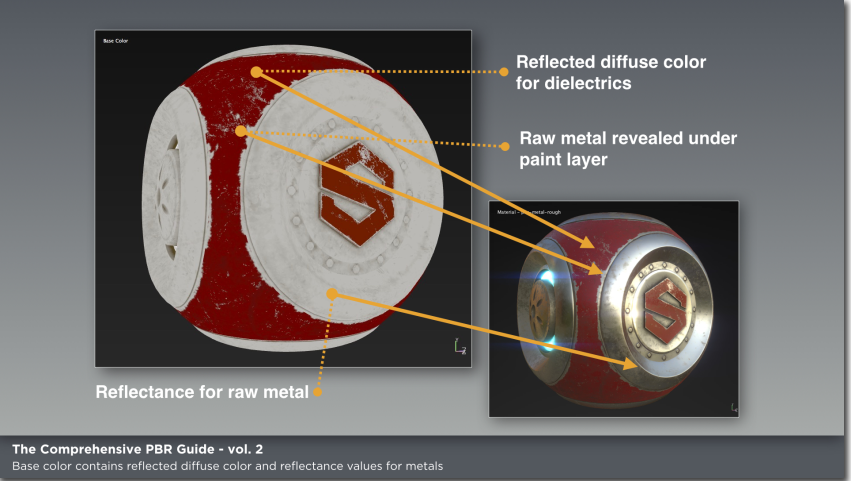
\includegraphics[width=\textwidth]{images/chap2_7.png}
	\caption{固有色贴图包含绝缘体的反射颜色和金属的反射率}
    \label{fig:chap2_7}
\end{figure}

\subsubsection{制作指导}

固有色贴图从色调上看应该是比较“平”的,譬如说和传统漫反射贴图相比对比度更低:里面的值不应该过大或过小。物体实际上会比我们觉得的颜色更亮一些。具体来说,我们想象一个最暗的东西——煤和最亮的东西——干净的雪。实际上煤并不是值为0的黑。我们需要使用范围内的颜色,实际上这里指的就是绝缘体的反射颜色。在图\ref{fig:chap2_8}里,你可以看到脏的部分比正确范围还要小的错误例子。就算是暗的地方也不应该低于sRGB下30-50。暗部在宽松限制下不应该低于sRGB 30,严格来说不能低于sRGB 50。对于亮的地方,sRGB不应该超过240。

我们前面已经提到固有色包含了根据绝缘体材质得到反射光,因此这里面应当去掉注入AO等光源信息。当然也有例外:当shader只用AO无法表达足够多细节时,可以加一些小的遮挡来提神效果。固有色中对应金属反射率的值应当从现实测量数据中得到。这些值一般在specular的70-100\%,对应sRGB范围是180-255。在后面的PBR Utilities一节中,我们会讨论提供了常见材质预制F0的工具。另外Sébastien Lagarde提供的金属度/粗糙度表格也是一个非常棒的参考资源。

https://seblagarde.wordpress.com/2014/04/14/dontnodphysically-based-rendering-chart-for-unreal-engine-4/

\begin{figure}[ht]
    \centering
	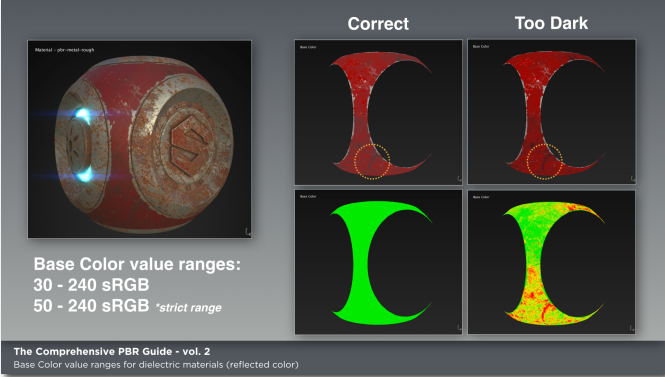
\includegraphics[width=\textwidth]{images/chap2_8.png}
	\caption{绝缘体的固有色范围}
    \label{fig:chap2_8}
\end{figure}

\textbf{金属反射率的值应当从现实测量数据中得到。}

\begin{enumerate}
\item 贴图颜色表示非金属的固有色和金属的反射率
\item 固有色应当避免颜色信息,但是可以有一些小AO
\item 暗部不应该低于sRGB 30(宽松限制)-sRGB 50(严格限制)
\item 亮部不应该超过sRGB 240
\item 金属反射率一般在specular的70-100\%,对应sRGB范围是180-255
\end{enumerate}

我们将在下面的金属度章节讨论到固有色也包含了金属反射值。如果在固有色里加上了尘土或氧化效果,就会导致金属反射值低于原始金属的对应范围。另外在金属度贴图上也需要进行修改:对应的值也需要低于原始值。例如图\ref{fig:chap2_10}中沾染了尘土的金属被当作绝缘体处理,因此金属度贴图中使用了黑色。

\textbf{金属度贴图用起来像一个遮罩层,告诉shader贴图的值对应金属反射值还是非金属固有色}

\begin{figure}[ht]
    \centering
	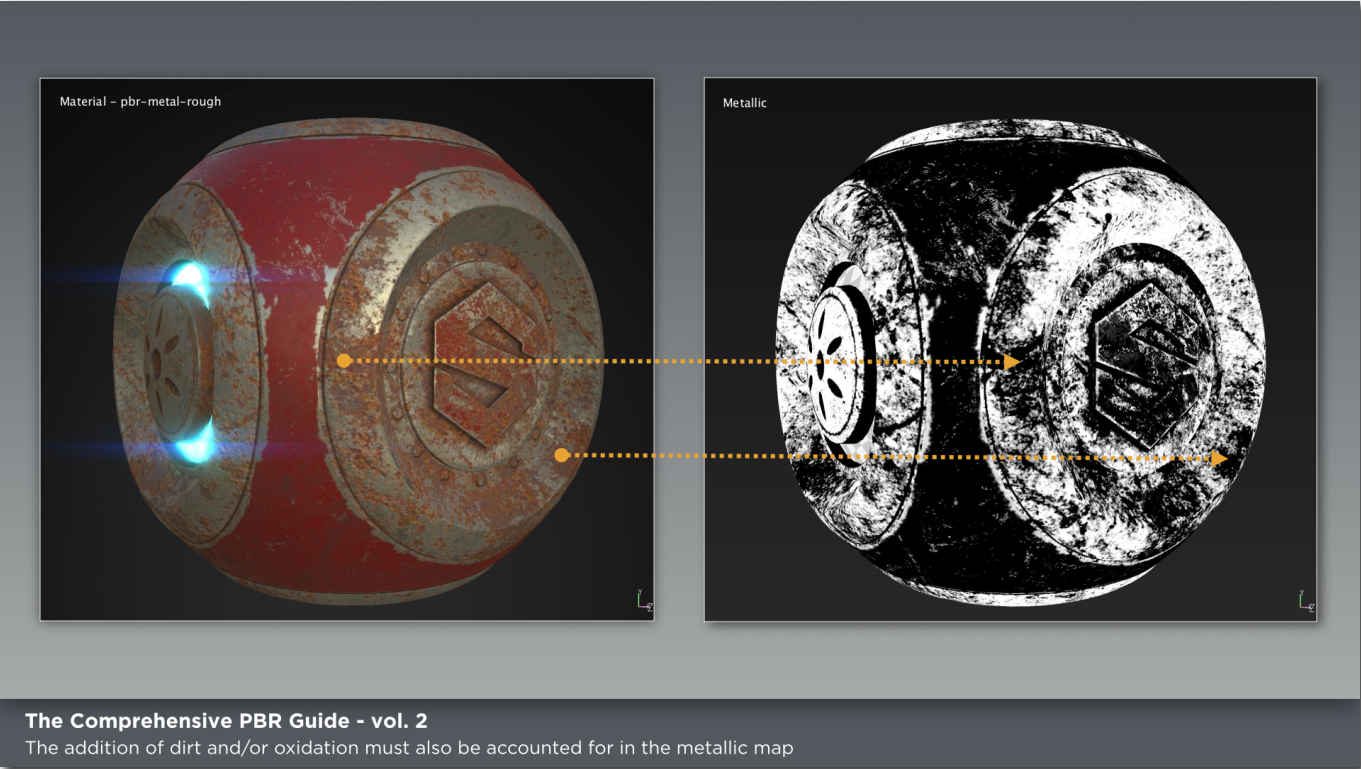
\includegraphics[width=\textwidth]{images/chap2_10.png}
	\caption{氧化效果和尘土需要在金属度贴图上也进行修改}
    \label{fig:chap2_10}
\end{figure}

\subsection{金属度 (灰度-线性)}

金属度贴图用来定义材质的哪些部分是金属。它是一张灰度图。金属度贴图用起来像一个遮罩层,告诉shader贴图的值对应金属反射值还是非金属固有色。它里面的数据并不包含真实世界数据,只是用来告诉shader固有色贴图应当被当作反射颜色(绝缘体)还是金属反射值使用。在贴图里,0.0(黑色-0 sRGB)表示非金属,1.0(白色-255 sRGB)表示金属。从区分金属和非金属的角度来说,金属度贴图一般是二元的,也就是说白色或黑色的。以图\ref{fig:chap2_11}为例,当shader发现金属度贴图是白色时,它会获取对应固有色贴图并将其作为金属反射率使用。

\begin{figure}[ht]
    \centering
	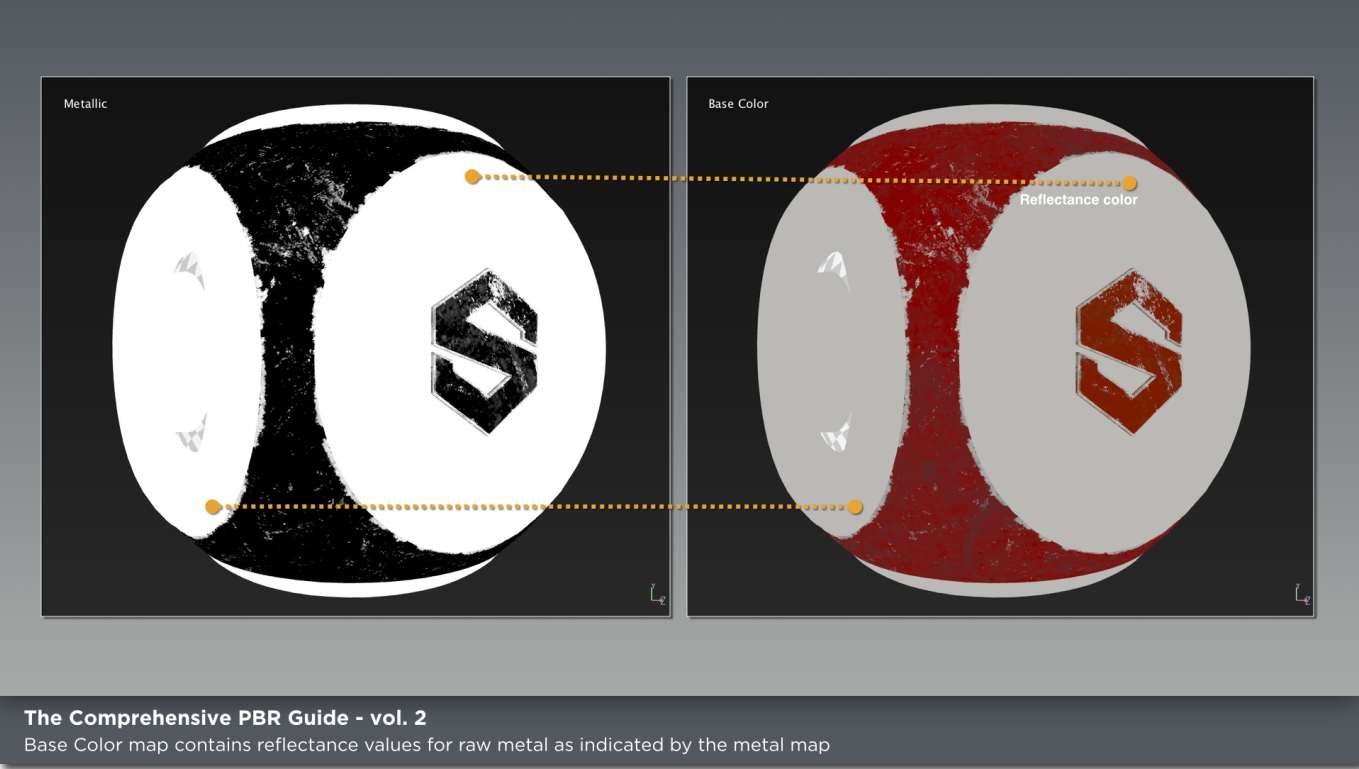
\includegraphics[width=\textwidth]{images/chap2_11.png}
	\caption{金属度贴图指定固有色贴图中的反射率部分}
    \label{fig:chap2_11}
\end{figure}

\subsubsection{制作指导}

对金属表面制作贴图的时候有两个重要的方面:一个是反射值应该比较高,在70-100\%范围;另一个是有些金属会被侵蚀。我们将在讨论制作指导的时候分别讨论。

\textbf{对这部分范围的金属区域来说,他们的反射率应当在70-100\%}

\paragraph{金属原材料}

金属度贴图应当被定义为0或1,也就是金属或非金属。这张图是用来定义擦亮的金属状态。作为一个通用的指导,金属原材料的灰度值应当是sRGB 235-255。对这个范围内的金属区域,应当有70-100\%的反射率区间,也就是在固有色贴图中对应sRGB 180-255,如图\ref{fig:chap2_12}所示。再一次需要强调的是,这些值应当都基于真实世界的测量数据。

\begin{figure}[ht]
    \centering
	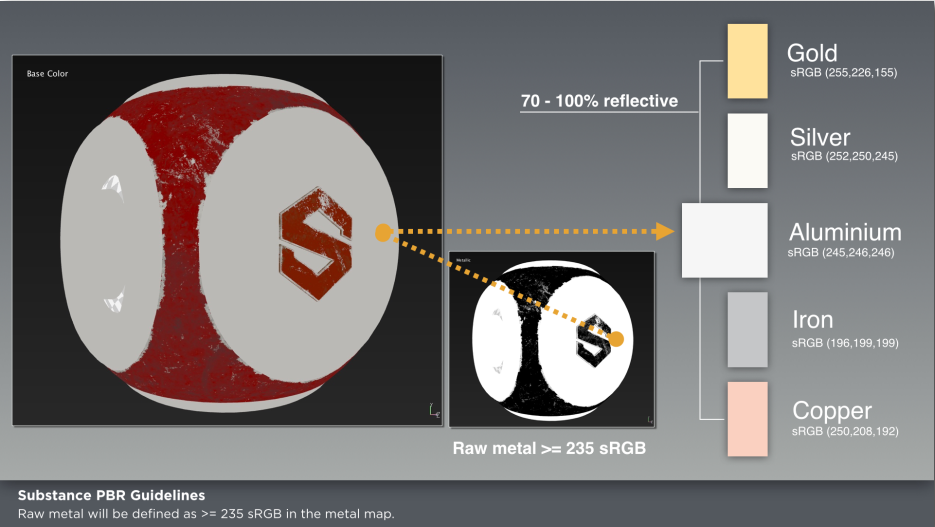
\includegraphics[width=\textwidth]{images/chap2_12.png}
	\caption{金属度贴图上原始金属的sRGB应当大于235}
    \label{fig:chap2_12}
\end{figure}

\paragraph{腐蚀或绝缘层}

当平面出现风化时,金属需要考虑氧化或受到诸如尘土或尘垢等环境因素影响。氧化部分的金属应当被处理成绝缘体,例如生锈的金属。油漆涂上的部分也是同理。图\ref{fig:chap2_13}中油漆部分中的划痕部分金属被暴露成原材料(金属图贴图中白色),而油漆是绝缘体(金属图贴图中黑色)。

\begin{figure}[ht]
    \centering
	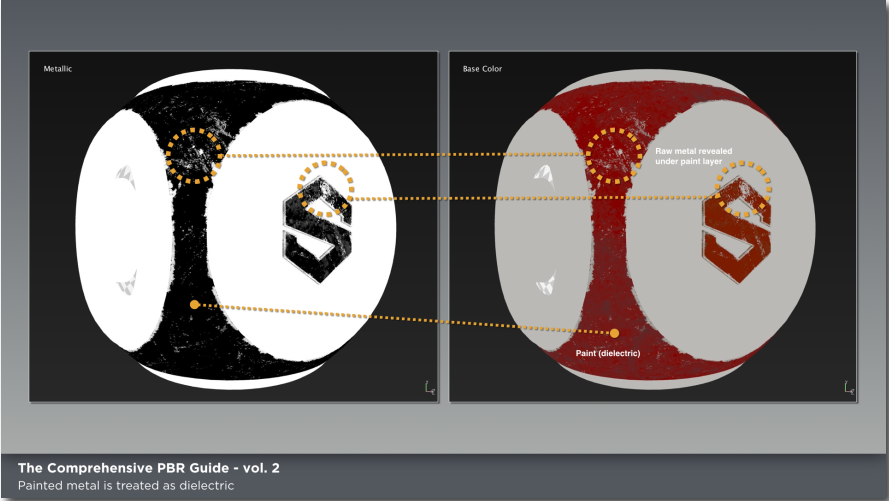
\includegraphics[width=\textwidth]{images/chap2_13.png}
	\caption{被颜料覆盖的金属被视为绝缘体}
    \label{fig:chap2_13}
\end{figure}

金属度贴图能通过灰度渐变表达金属和非金属间的混合状态。关键点在于如果金属度贴图的灰度值低于sRGB 235,那么对应固有色贴图中的『原始』金属反射值需要降低。举个例子,图\ref{fig:chap2_14}中有一层尘土部分遮挡了金属。这层尘土是绝缘的,如果你在金属度贴图中没有单独处理的话,那么尘土对应的固有色贴图就会被当成金属反射率使用。同时尘土的颜色会比光滑金属对应的70-100\%反射率低很多。正确的做法是降低金属度贴图中尘土对应的部分,这样就能得到一个正确的绝缘部分和金属反射率之间的混合效果。

尘土层的透明度能够用来表明固有色中的反射率应该降低多少。这里没有什么明确无误的规则。你要做的是从一个高反射率(金属)过渡到低反射率(绝缘体)。具体下降多少要根据使用场景而定。

Substance工具能帮助你更轻松的实现这些效果,并通过多个通道来控制这些效果的度。Substance Designer和Substance Painter能使你调整Substance效果的参数,这将自动调整对应的通道。例如在Substance Designer里,你可以使用一个颜色混合节点来实现多个通道的尘土效果。如图\ref{fig:chap2_15}所示,你可以通过金属度滑杆来调整金属上覆盖的尘土层效果。

\begin{figure}[ht]
    \centering
	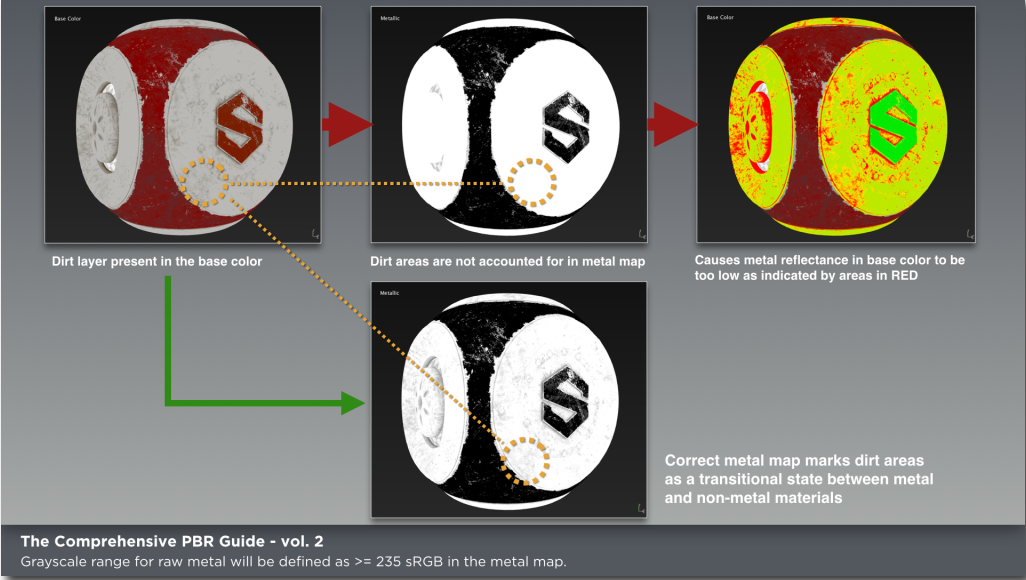
\includegraphics[width=\textwidth]{images/chap2_14.png}
	\caption{金属度贴图中金属部分对应值应当不小于sRGB 235}
    \label{fig:chap2_14}
\end{figure}

\textbf{被氧化的金属应该被当做绝缘体,如生锈部分。被油漆覆盖的同理。}

\begin{figure}[ht]
    \centering
	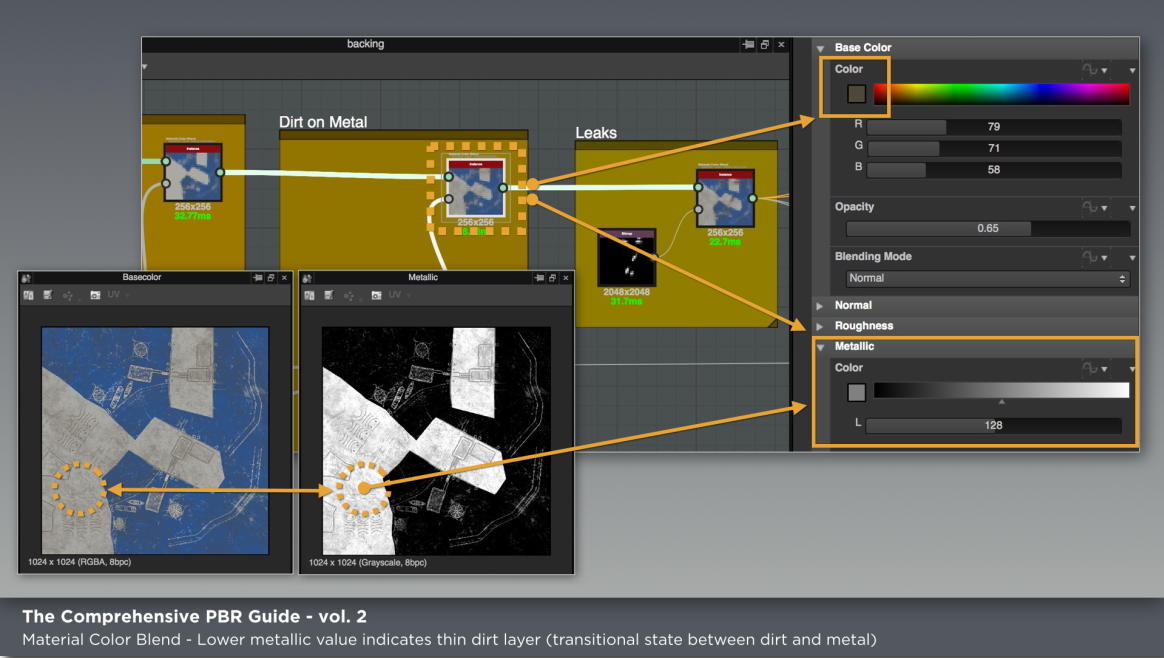
\includegraphics[width=\textwidth]{images/chap2_15.png}
	\caption{材质颜色混合-更低的金属度意味着薄尘土层(金属和尘土之间的状态)}
    \label{fig:chap2_15}
\end{figure}

\begin{enumerate}
\item 黑色(0.0)表示非金属,白色(1.0)表示金属。中间的过渡值能用来表示氧化或者尘土。
\item 如果金属度对应值小于235 sRGB,那么固有色贴图中的反射率需要降低。
\end{enumerate}

\subsection{粗糙度 (灰度-线性)}

粗糙度贴图描述平面的不规则程度,这个导致了图\ref{fig:chap2_16}中的光扩散的效果。正如券一所讨论,平面粗糙能导致光随机反射。这个导致光的方向发生变化,但是光的强度保持不变。粗糙的平面对应的是更大且更暗的高光;光滑的平面将保持高光反射狙击,这意味着看起来更亮(虽然反射的光总量是相同的)。

在粗糙度贴图中,黑色(0.0)表示光滑的平面,白色(1.0)表示粗糙的平面。粗糙度贴图实际上是最有创造性的,因为它使得艺术家能够可视地定义表面的特征。从本质上来说,它甚至允许你创造性的编故事来描述表面情况:这个表面周围的环境是怎么样的?它是被小心翼翼的保护着还是随手扔在一边?有没有经过时间的洗礼?这些能够告诉我们很多环境信息,进一步来说和整个素材的设计及创建的世界联系起来。

就粗糙度来说,没有明确的对或者错。艺术家拥有全部的控制权。一个比较好的出发点是法线贴图:法线贴图一般都包含了关键的表面信息,而这些也需要在粗糙度贴图中表达出来。

\begin{figure}[ht]
    \centering
	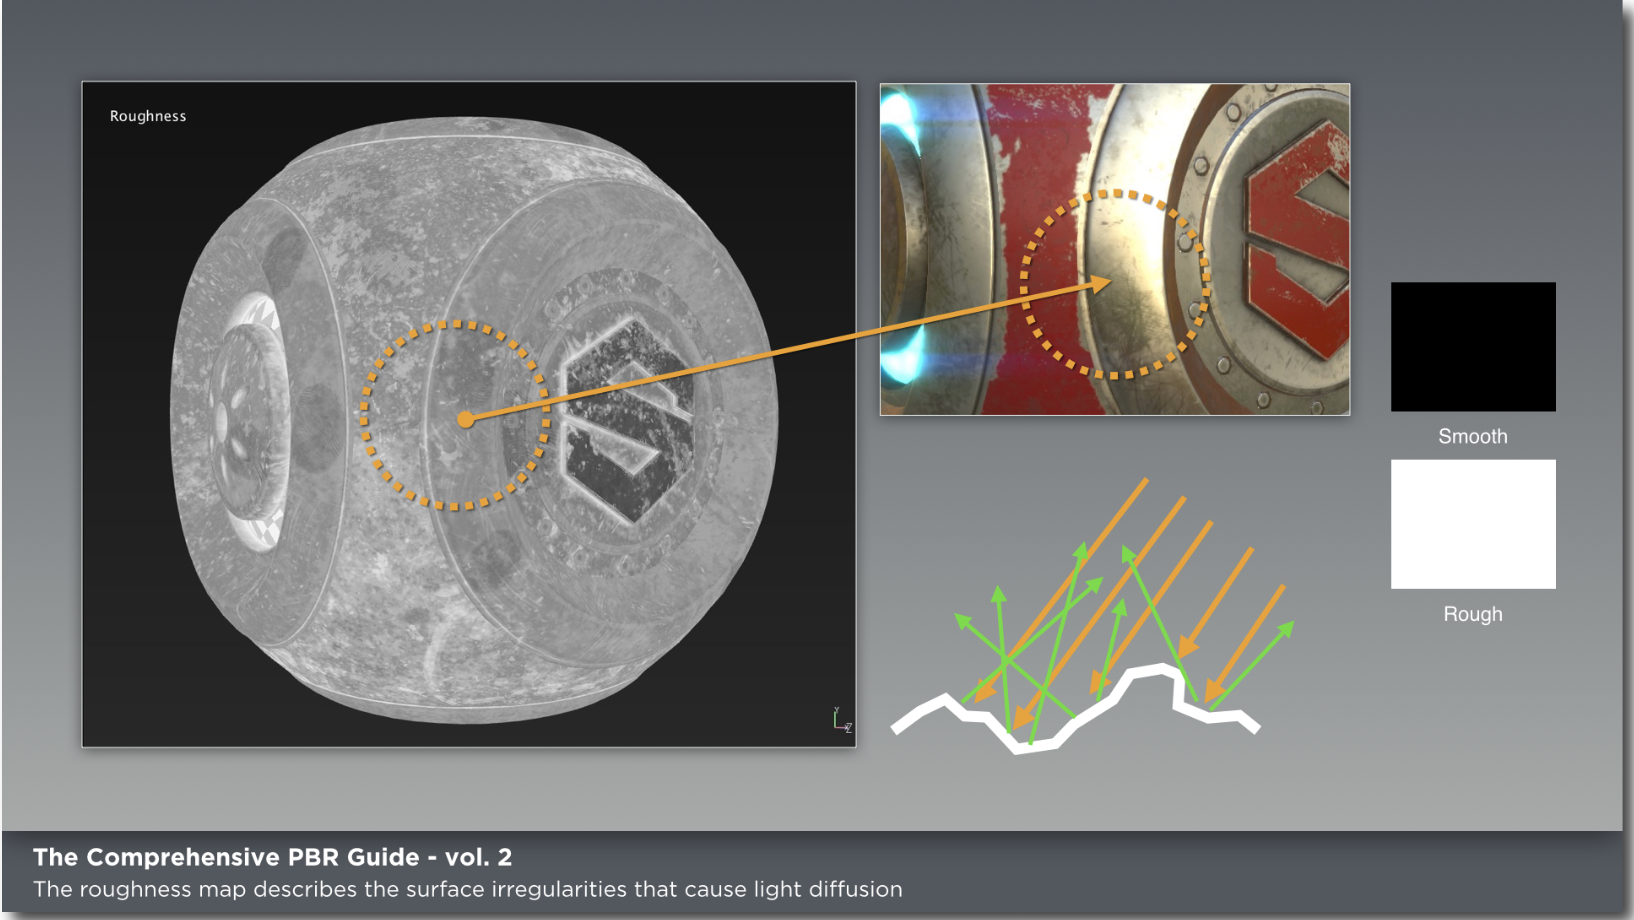
\includegraphics[width=\textwidth]{images/chap2_16.png}
	\caption{粗糙度贴图描述平面的不规则程度,这导致了光的扩散}
    \label{fig:chap2_16}
\end{figure}

\subsubsection{制作指导}

\begin{enumerate}
\item 富有创造力地描述一个关于平面的故事。
\end{enumerate}

\subsection{分辨率与纹理元素密度}

金属度/粗糙度的一个副产物是可能产生白边瑕疵,如图\ref{fig:chap2_17}所示。虽然我们正在讨论的是金属度工作流,但这个问题也会出现在高光/光滑度工作流中。但那种情况下就不会非常显眼,因为会倒过来成为黑色边缘,如图\ref{fig:chap2_18}。

在不同材质的交接区域能够看到很明显的缝隙,如图\ref{fig:chap2_19}中从绝缘体到一个非常亮的金属的插值部分。在金属度/粗糙度工作流中,金属的固有色部分由于和非金属的漫反射颜色插值,因此会比其反射率高,交界处产生白色。在高光/光滑度工作流中,金属没有漫反射颜色因此对应黑色。这个黑色的值和非金属的漫反射颜色插值,于是产生了一个黑色的边缘。

贴图分辨率和纹理密度对边缘瑕疵有直接影响。譬如当你使用一个硬边的刷子来创建金属和非金属的交界区域时,贴图分辨率较低的话边缘就会被软化,加剧瑕疵。这个低分辨率的问题也会由于UV不当产生:即使整体分辨率足够,但对应的纹理密度太低。

\textbf{贴图分辨率和纹理密度对边缘瑕疵有直接影响。}

\begin{figure}[ht]
    \centering
	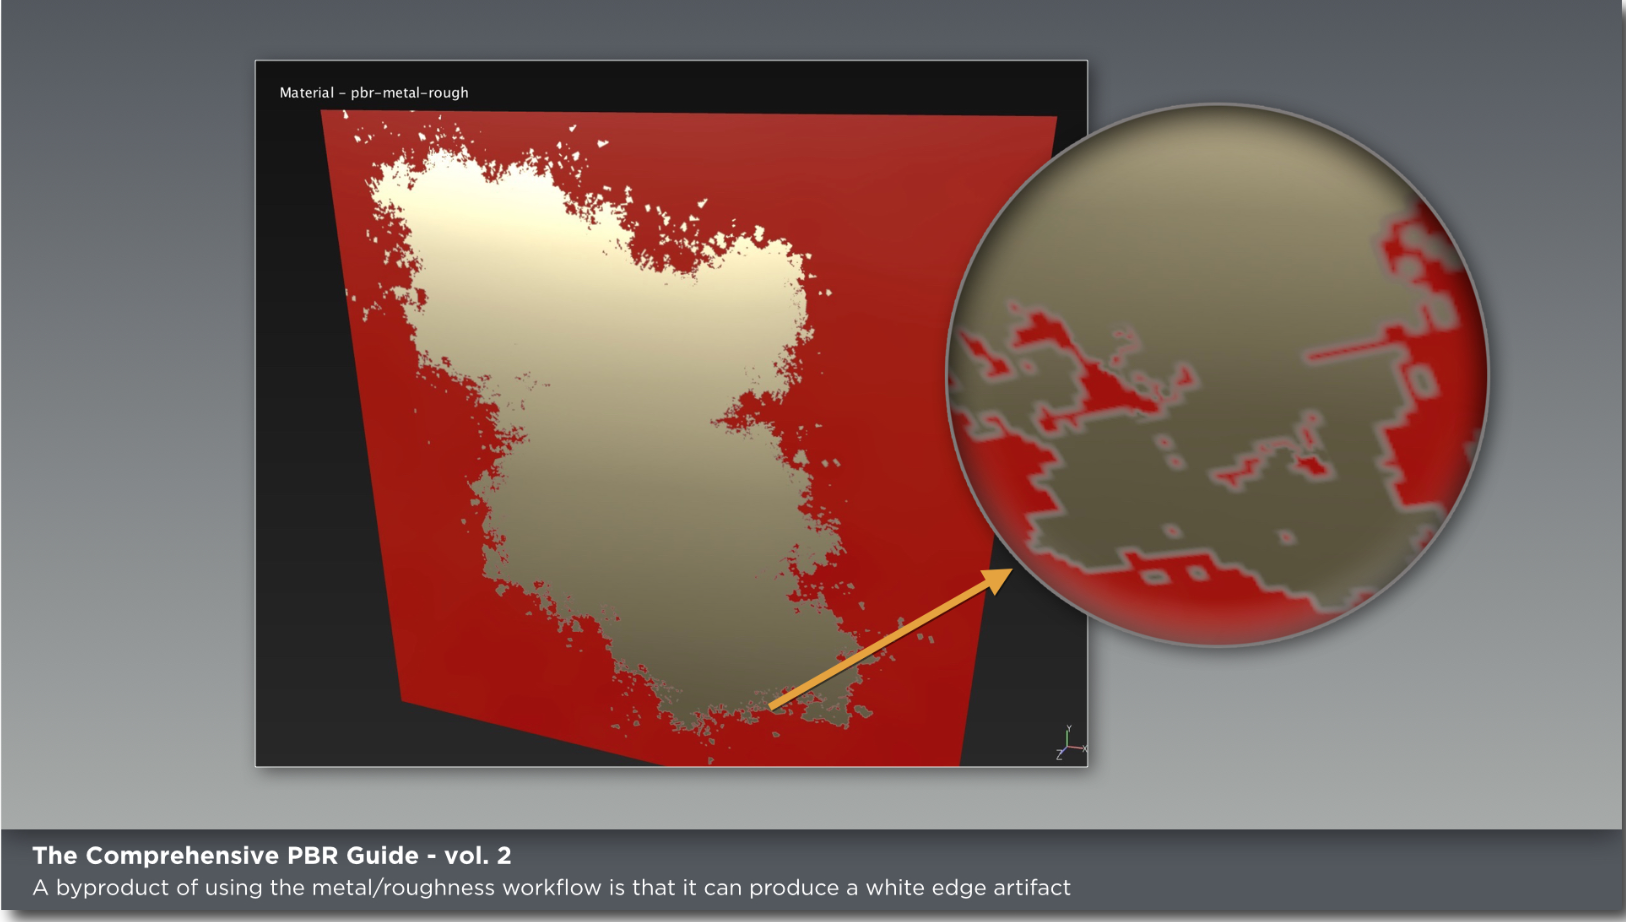
\includegraphics[width=\textwidth]{images/chap2_17.png}
	\caption{金属度/粗糙度工作流带来的副产品:白色边缘瑕疵}
    \label{fig:chap2_17}
\end{figure}

\begin{figure}[ht]
    \centering
	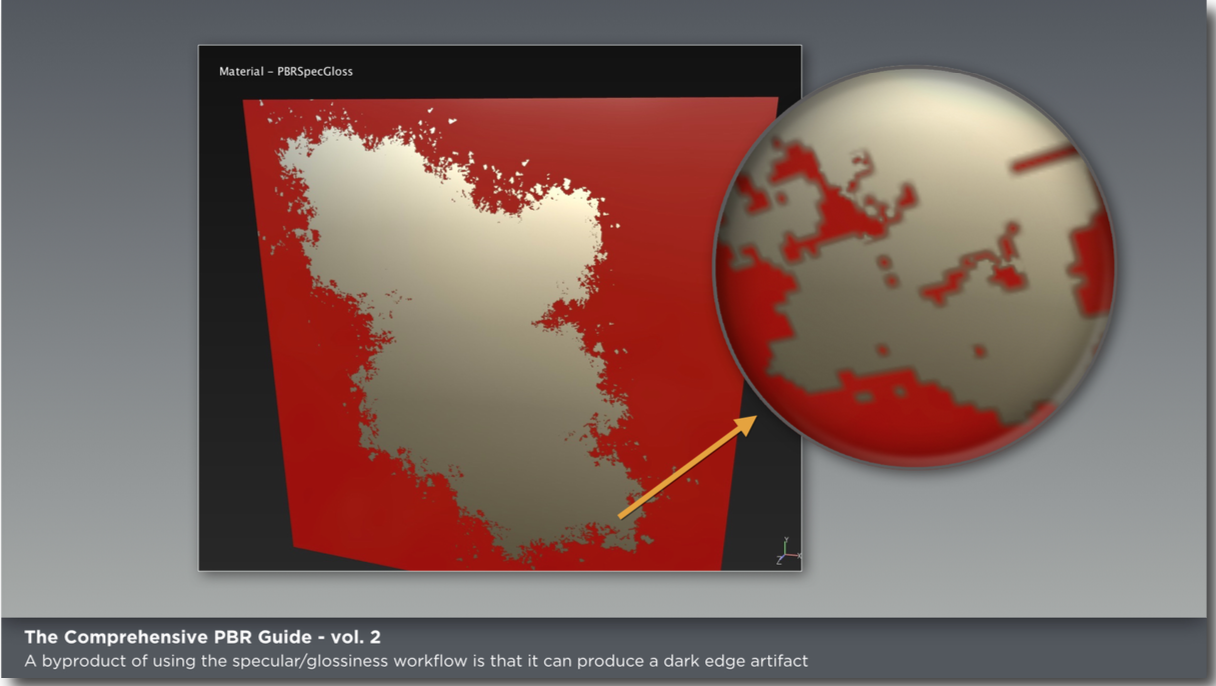
\includegraphics[width=\textwidth]{images/chap2_18.png}
	\caption{高光/光滑度工作流的副产品是黑色边缘瑕疵}
    \label{fig:chap2_18}
\end{figure}

\begin{figure}[ht]
    \centering
	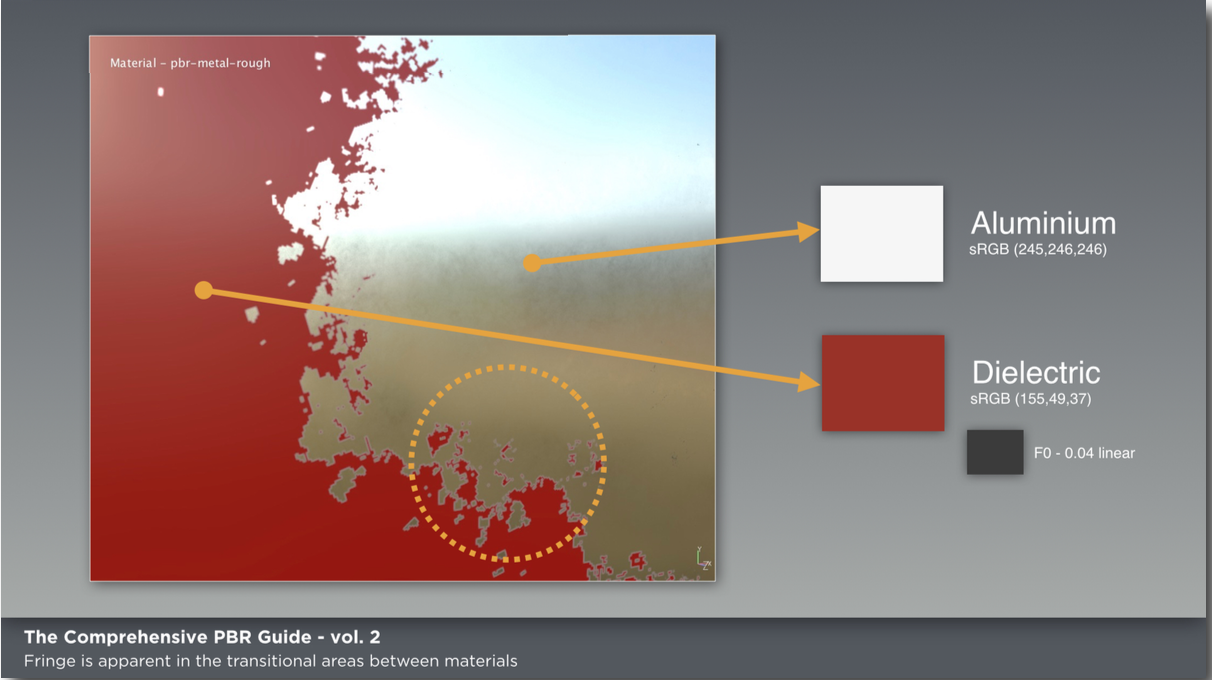
\includegraphics[width=\textwidth]{images/chap2_19.png}
	\caption{在不同材质交界处能明显看到边缘}
    \label{fig:chap2_19}
\end{figure}

\subsubsection{制作指导}

\begin{enumerate}
\item 纹理元素密度和分辨率会影响金属度/粗糙度工作流中出现白边。确认UV分配合适,保证足够的纹理密度来减轻瑕疵。
\end{enumerate}

\subsection{高光}

金属度/粗糙度工作流中绝缘体材料的F0一般都是线性0.04。正如前面所说,一些实现允许你通过高光项覆盖这个设置。在Substance里提供了一个高光等级的通道。由于绝缘体F0使用在创作规范上比较复杂,而且大多数金属度/粗糙度工作流也只用0.04这个值,我会等到讨论高光/光滑度工作流的时候再来讨论这块的使用。

\subsection{金属度/粗糙度工作流的优缺点}

\textbf{优点}

\begin{enumerate}
\item 创作者使用更加简单,避免由于提供错误的绝缘体F0数据带来的问题
\item 使用了更少的贴图大小,这是因为金属度和粗糙度都是灰度图
\item 看上去是一种被更加宽泛采纳的工作流
\end{enumerate}

\textbf{缺点}

\begin{enumerate}
\item 无法通过贴图来控制绝缘体F0。当然大多数实现能够覆盖默认的4\%值。
\item 低分辨率下边缘的瑕疵更容易被发现。
\end{enumerate}

视频介绍在\href{http://www.allegorithmic.com/pbr-guide}。

\section{高光/光滑度工作流}

与 金属度 / 粗糙度类似,高光 / 光滑度工作流使用一系列贴图(maps)控制相关的参数,并将这些贴图以纹理(textures)的方式提供给PBR shader的采样器(sampler)进行读取。如图21所示,高光 / 光滑度工作流使用的贴图包括:漫反射贴图(diffuse)、高光贴图(Specular)和光滑度贴图(Glossiness)。尽管高光/光滑度工作流中使用的贴图名字(例如漫反射,高光等)听起来和传统贴图的名字类似,但是这些贴图与传统工作流中那些同名贴图是不一样的,请一定注意对他们加以区分。在Substance中,我们会使用“漫反射”(diffuse)这个名词,而其他的PBR实现中可能会管漫反射这个词叫“漫反射率”(Albedo)。PBR shader还会使用之前提过的环境光遮蔽(Ambient Occlusion),法线(Normal),还有可能用到视差映射(parallax mapping);这些相关事项会在后面的“两个流水线常用的贴图”一节讲到。

在高光 / 光滑度工作流中,金属度的镜面反射比(reflectance value)和非金属材质F0的值需要被放到高光贴图(specular map)里。若要使用高光 / 光滑度工作流,你需要两个RGB贴图:一个存漫反射“颜色”(漫反射率),另一个存镜面反射比。同时对于非金属,高光贴图存的是非金属物质F0数据。

正如我们在前文中讲金属度/粗糙度工作流时所提到的,Substance系列软件中的PBR shader需要确保能量保守(Energy Conservation),这一点在高光 / 光滑度工作流中变的更为重要。在高光 / 光滑度工作流中,决定非金属F0值的高光贴图是由人决定的\footnote{译者注:而不是由metallic值算出来的,因此更容易因为人的因素而产生错误}。举个例子,若一个材质是由一个纯白色(1.0f)的漫反射贴图加一个纯白色(1.0f)的高光贴图组成的,那么这个材质反射出的光照强度就会比他接受到的光照强度还要大,能量保守的原则就被破坏了。当你使用这套纹理时,这套纹理将不能反映真实材质的视觉效果。

通过下面的介绍你会发现,高光/光滑度工作流中贴图所表达的材质属性数据实际上与金属度/光滑度贴图是一样的。因此,在使用这两种工作流制作素材时所遵循的指导原则是一样的,只不过在处理贴图内容的时候会有些不同。材质的各种属性数据会在遵守相同原则的基础上被放到不同的贴图里。前文提到,所有的这些材质的属性数值(包括非金属F0、金属反射比和漫反射率的值)都来自于实测数据。在本指导手册里讨论过的这些不同种类的贴图数据均基于实测数据。在这一节里,我们将不会重复金属度 / 粗糙度工作流部分里面提过的某些内容,而更加关注两个工作流之间的差别以及使用高光 / 光滑度工作流时所需要注意的事项。

\subsection{漫反射(RGB-sRGB)}

与前面金属度/粗糙度工作流中的固有色贴图(base color map)一样,漫反射贴图存储的是物体的漫反射率。但是,在这高光 / 光滑度工作流中,这张漫反射贴图不包含任何镜面反射比(reflectance value)数据。

\subsubsection{制作指导}

漫反射贴图里面只存漫反射率。在图22中,漫反射贴图中映射纯属(raw metal)区域的漫反射值是黑色的(0.0f),因为金属没有漫反射颜色。对于氧化了的金属,这些金属所对应的区域是有漫反射颜色的,因为这些区域已经不能被当做纯金属对待了。同理,纯金属上覆盖的灰尘泥巴也会在金属上形成非金属层。\footnote{译者注:从而使得这些区域对应的漫反射贴图变得有颜色}

\begin{enumerate}
\item 漫反射贴图中带颜色的区域对应的是非金属材质,纯黑(0.0f)的区域对应纯金属材质。
\item 除了微观层面上遮蔽所产生的颜色变暗,漫反射的颜色应该避免包含任何光照信息。
\item (在0-255范围,sRGB模式下)漫反射率绝对不能低于30,最好不低于50,。金属区域的黑色除外。
\item (在0-255范围,sRGB模式下)漫反射率最大不能高于240。
\end{enumerate}

\subsection{高光反射(RGB-sRGB)}

高光贴图定义了金属的镜面反射比和非金属的F0值,如图23所示。这张RGB贴图内可以存储各种不同的非导电物质所特有的值\footnote{译者注:F0值}。这和金属/粗糙度工作流中的方法不太一样,后者的非金属的F0值被硬编码成4\%并且只能通过镜面反射度通道(specular level)来改变。正如之前金属/粗糙度工作流里那样,F0的数据需要来自真实测量得到的数值。非导电物质的F0是单通道灰度值,而金属的镜面反射比是带颜色的。这是由于某些金属对不同波长的光波(不同颜色)吸收程度不一样造成的。

\textbf{镜面反射贴图里可以为不同的非导电体存储不同的F0值。}

\subsubsection{制作指导}

因为高光贴图包含了金属与非金属两类物质的F0值,我们将把贴图的内容按照物质的属性拆成两部分。

\paragraph{纯金属}

F0需要基于真实世界的数据。就像我们在金属度贴图中提到的一样,如果纯金属的表面有氧化或者表面有非金属物质的覆盖层,那么金属的镜面反射率数值就要(比纯金属的时候)小一些。高光/光滑度工作流中,表面灰尘或者氧化会增加纯金属表面漫反射率贴图的反射率并减高光贴图中的镜面反射比,如图24所示。该图中还展示了一个带灰尘纯金属表面的例子。高光贴图中灰尘的F0值根据非金属物质的F0来确定,使用0.04或4\%。

\paragraph{绝缘体}

绝缘体的F0值同样也存在于高光贴图中。在这种情况下你可以完全控制F0值的大小,注意这个值一定要基于真实数据。如我们在第一本书中所提到的,非金属(绝缘体,非导电物质)导电性能不佳。因此,折射光线在非金属物体表面会散射或者被吸收(不过通常会从物体表面发散出来)从而使得镜面反射出来的光强度远远小于金属物质。根据物质折射率计算得到的结果,常见非导电物质的F0一般在2-5\%之间。除了矿物宝石类物质之外,大多数非导电物质的F0值大概处于0.02-0.05(线性采样值)之间,如图25所示。若用sRGB表示,值大概在sRGB40-75左右,这一段数值转换成0到1之间的值大概在0.02-0.05之间。

如果你找不到某种特定物质的折射率,则F0值可以被定为4\%(0.04-塑料)。矿物宝石是一个例外,其值大约为0.05-0.17(线性采样值)之间,如图21所示\footnote{译者注:该处图编标号疑有错误,应为图25}。

\begin{enumerate}
\item 高光贴图保存了非导电物质的F0和纯金属的镜面反射比。
\item 非金属的镜面反射光强度小于金属的镜面反射率。非金属的F0值一般在2-5\%之间(sRGB值),若用sRGB表示其范围为40-75之间,对应0.02-0.05(线性采样值)范围。
\item 一般的矿物宝石类物质的F0在0.05-0.17(线性采样值)之间。
\item 大多数的液体F0在0.02-0.04(线性采样值)之间。
\item 金属物质的镜面反射比一般很高,早70\%-100\%之间,转换成sRGB值大概就是180-255之间。
\item 如果某种物质的折射率查不到,可以使用4\%这个值(0.04-塑料)。
\end{enumerate}

\subsection{光滑度(灰度-线性采样)}

光滑度贴图描述了物体表面的不规则度(如图26所示),这种不规则会使得反射光线模糊。在这张贴图中,黑色(0.0f)代表粗糙的表面,白色(1.0f)代表光滑的吧表面。这张图的内容是金属度/粗糙度工作流中粗糙度贴图的反相(Inverse)。这张贴图的制作指导与之前粗糙度贴图部分的制作指导相同。

\textbf{描述了物体表面会导致反射光模糊的物体表面不规则度。}

\subsubsection{制作指导}

\begin{enumerate}
\item 发挥想象力,用这张贴图视觉化地表现物所经历过的世间种种。
\end{enumerate}

\subsection{分辨率与纹理元素密度}

在前文中我们讨论了会出现在两个工作流中的纹理边缘瑕疵问题。由于这个问题在金属度/粗糙度工作流中跟家明显,所以这个问题在金属度/粗糙度部分详细的讨论过。在本工作流中这一问题同样值得注意:由于金属没有漫反射率颜色。金属区域的漫反射颜色会和与其接壤的非金属区域漫反射颜色进行插值,从而产生如图27所示的黑边。

在此我们再提一次,贴图文件的分辨率和纹理元素密度会直接作用并影响纹理边缘问题的出现。例如,你的物体有一部分是用较硬的笔刷绘制的金属与非金属接壤处,那么分辨率比较小小的贴图文件会软化这个原本很硬的边缘,加重纹理边缘瑕疵的问题。分辨率过低的问题还有可能是因为UV区域没有映射足够多的纹理元素。让UV覆盖足够多的纹理元素是解决这个问题的最好办法。(如图28所示)

\textbf{文档的分辨率和纹理元素密度会直接影响纹理边缘瑕疵的严重程度。}

\subsubsection{制作指导}

\begin{enumerate}
\item 纹理元素和贴图分辨率会影响高光/光滑度工作流中出现的黑边问题。为了减缓黑边问题,请让UV覆盖足够多的纹理元素。
\end{enumerate}

\subsection{高光/光滑度工作流的优缺点}

优点:

\begin{enumerate}
\item 边缘瑕疵问题不那么明显。
\item 可以控制非金属物体的F0。\footnote{译者注:在某些引擎的PBR实现中,如Unity的Alloy Shader和UE4中,金属度/粗糙度工作流中的F0也可以通过外部输入控制。}
\end{enumerate}

缺点:

\begin{enumerate}
\item 由于高光贴图完全控制非金属F0,因此更有可能因为人为原因使得该值错误,进而破坏能量保守。
\item 会额外多使用一个RGB通道的贴图。\footnote{译者注:高光贴图,金属度/粗糙度工作流中金属度只要单通道就可以表示}
\item 使用的名词与传统流程中的流程名词相似,但是所指的东西完全不是一回事儿。同时需要扎实的基于物理光照的知识和概念才能将贴图画对。例如:F0不能瞎填要基于真实数据,纯金属的漫反射要是黑的。
\end{enumerate}

\section{不同工作流共用贴图}
\label{sec:common_maps}

\section{Substance PBR功能}